\documentclass[conference]{IEEEtran}
\IEEEoverridecommandlockouts
\usepackage{cite}
\usepackage{amsmath,amssymb,amsfonts}
\usepackage{algorithmic}
\usepackage{graphicx}
\usepackage{float}
\usepackage{textcomp}
\usepackage{xcolor}
\usepackage{url}
\usepackage[spanish,es-nodecimaldot]{babel}
\usepackage[utf8]{inputenc}
\usepackage{textgreek}
\usepackage{booktabs}

\def\BibTeX{{\rm B\kern-.05em{\sc i\kern-.025em b}\kern-.08em
    T\kern-.1667em\lower.7ex\hbox{E}\kern-.125emX}}

\begin{document}

\title{Clasificación Automática de Subgéneros de Jazz\\mediante Machine Learning y Deep Learning}

\author{
\IEEEauthorblockN{Benjamín Ferrada Larach}
\IEEEauthorblockA{Universidad Técnica Federico Santa María\\
Valparaíso, Chile\\
benjamin.ferradal@usm.cl}
}

\maketitle

% ============================================================
\begin{abstract}
Este proyecto aborda la clasificación de grano fino de subgéneros musicales dentro de la categoría Jazz utilizando el dataset FMA (\textit{Free Music Archive}). Se diseñó e implementó un pipeline dual para comparar un algoritmo tradicional (Random Forest sobre características tabulares) frente a una arquitectura profunda (Red Neuronal Convolucional sobre espectrogramas de Mel). Los principales desafíos técnicos —desbalanceo extremo de clases y escasez de datos etiquetados de forma específica— fueron abordados mediante sobremuestreo sintético (SMOTE), regularización L2, reducción de capacidad de la red y eliminación de pesos de clase en la CNN. Los resultados finales muestran que la CNN optimizada alcanza una exactitud del 76\%, superando al Random Forest (72\%). La combinación de ambos mediante un ensamble de votación suave ponderada logra un F1-macro de 0.71, con una precisión del 92\% en la clase Free-Jazz. Estas cifras demuestran que las representaciones espectro-temporales capturan matices acústicos que los descriptores estacionarios no logran representar, aunque el tamaño reducido del corpus limita la generalización de la CNN en clases minoritarias.
\end{abstract}

\begin{IEEEkeywords}
Clasificación de Audio, Deep Learning, Jazz, Redes Convolucionales, Random Forest, SMOTE, Regularización L2.
\end{IEEEkeywords}

% ============================================================
\section{Introducción y Definición del Problema}

La Clasificación de Información Musical (MIR, por sus siglas en inglés) ha resuelto en gran medida la categorización a nivel macro (e.g., distinguir entre Rock y Música Clásica). Sin embargo, la clasificación intra-género o de \textit{grano fino} presenta una frontera de investigación activa. Subgéneros del Jazz, tales como el \textit{Bebop}, \textit{Swing} o \textit{Free-Jazz}, comparten de forma inherente la misma instrumentación y progresiones armónicas similares, diferenciándose sutilmente por el fraseo, la síncopa y la disonancia intencional \cite{b1}.

El problema abordado es la automatización de esta categorización utilizando un corpus de audio de tamaño mediano (FMA Medium, 22 GB en su forma original). Además de la similitud acústica entre subgéneros, los datos del mundo real presentan un fuerte desbalanceo: la etiqueta genérica ``Jazz Genérico'' domina abrumadoramente sobre las específicas, propiciando el colapso predictivo (\textit{Mode Collapse}) de los algoritmos de aprendizaje si no son tratados adecuadamente. La combinación de estas dificultades convierte al problema en un caso de estudio representativo de los desafíos reales en MIR.

% ============================================================
\section{Descripción de los Datos}

\subsection{Dataset FMA}
Se utilizó el subconjunto FMA Medium \cite{b1}, que contiene pistas de audio en formato MP3 de 30 segundos. A partir del archivo original de 22 GB, se extrajeron selectivamente 614 pistas clasificadas bajo el género Jazz, reduciendo el tamaño en disco a aproximadamente 300 MB. Las pistas se distribuyen en seis subgéneros, cuyo desbalanceo natural se refleja en la Tabla~\ref{tab:distribucion}.

\begin{table}[htbp]
\centering
\caption{Distribución de pistas por subgénero (conjunto completo)}
\label{tab:distribucion}
\begin{tabular}{@{}lcc@{}}
\toprule
\textbf{Subgénero} & \textbf{Pistas originales} & \textbf{Tras aumento} \\ \midrule
Jazz Genérico      & 204 & 204 \\
Free-Jazz          & 133 & 399 \\
Modern Jazz        &  51 & 153 \\
Jazz: Out          &  44 & 132 \\
Jazz: Vocal        &  43 & 129 \\
Big Band/Swing     &  15 &  15 \\
\midrule
\textbf{Total}     & \textbf{490} & \textbf{1\,032} \\
\bottomrule
\end{tabular}
\end{table}

\subsection{Aumento de Datos en el Dominio del Audio}
Para mitigar el desbalanceo antes de la extracción de características, se aplicó \textit{Pitch-Shifting} directamente sobre la señal de audio cruda: cada pista de subgénero definido (excluyendo ``Jazz Genérico'') fue clonada en una versión aguda (+2 semitonos) y una versión grave ($-$2 semitonos) sin alterar el ritmo. La etiqueta de subgénero se conserva en los clones, triplicando efectivamente el número de ejemplos de las clases sub-representadas antes de la extracción de características.

% ============================================================
\section{Solución Propuesta e Implementación}

\subsection{Arquitectura del Pipeline}
La implementación se organiza en tres módulos secuenciales dentro del repositorio:

\begin{enumerate}
    \item \texttt{download\_data.py}: Descarga selectiva del archivo FMA Medium y extracción quirúrgica de los MP3 correspondientes al género Jazz, seguida de limpieza automática del ZIP original para recuperar espacio en disco.
    \item \texttt{extract\_features.py}: Procesamiento de señal y generación de las matrices de características en formato \texttt{.npy}, listas para ser consumidas por los modelos.
    \item \texttt{model.ipynb}: Entrenamiento, evaluación comparativa y ensamble de los modelos.
\end{enumerate}

\subsection{Extracción de Características}
Cada pista es cargada con \texttt{librosa} \cite{b2} a 22\,050 Hz y truncada a 30 segundos. El pipeline se bifurca en dos representaciones paralelas:

\textbf{Vector tabular (para Random Forest):} Se extrajeron 20 Coeficientes Cepstrales de las Frecuencias de Mel (MFCCs), sus deltas y delta-deltas, vectores \textit{Chroma}, \textit{Spectral Rolloff} y \textit{Zero Crossing Rate} (ZCR). El promedio temporal de cada descriptor genera un vector de 74 características que resume el timbre estático y la armonía subyacente. El ZCR es especialmente discriminativo para géneros caóticos como el Free-Jazz.

\textbf{Espectrograma de Mel (para CNN):} Se generó el espectrograma de Mel de 128 bandas, convertido a escala de decibelios y normalizado por instancia al rango $[0, 1]$ mediante:
\begin{equation}
S_{\text{norm}} = \frac{S_{\text{dB}} - \min(S_{\text{dB}})}{\max(S_{\text{dB}}) - \min(S_{\text{dB}}) + \epsilon}
\label{eq:norm}
\end{equation}
donde $\epsilon = 10^{-8}$ previene divisiones por cero en segmentos de silencio. La matriz resultante se redimensiona a $128 \times 128 \times 1$ para ser tratada como imagen por la CNN.

\subsection{Modelo Tabular: Random Forest con SMOTE}
Dado el desbalanceo residual tras el aumento de datos, se aplicó SMOTE \cite{b3} de forma dinámica: el número de vecinos $k$ se ajusta automáticamente al tamaño de la clase más pequeña ($k = \min(5,\, n_{\min} - 1)$), con un \textit{fallback} a \texttt{RandomOverSampler} si $n_{\min} < 2$. Tras el balanceo, las seis clases quedan igualadas a 204 muestras cada una en el conjunto de entrenamiento.

Los hiperparámetros del Random Forest se optimizaron mediante \texttt{RandomizedSearchCV} con 200 iteraciones y validación cruzada de 3 particiones, convergiendo en: \texttt{n\_estimators}=400, \texttt{max\_depth}=20, \texttt{min\_samples\_split}=5, \texttt{min\_samples\_leaf}=1, \texttt{bootstrap}=False.

\subsection{Modelo Profundo: CNN con Regularización L2}
La arquitectura original de tres bloques convolucionales fue rediseñada para adaptarse al tamaño reducido del corpus. Los cambios clave respecto a la versión inicial fueron: (1) reducción de la capacidad a la mitad (filtros 16-32-64 en lugar de 32-64-128), (2) regularización L2 con $\lambda = 10^{-3}$ en todas las capas convolucionales y densas, (3) sustitución de \texttt{Flatten} por \texttt{GlobalAveragePooling2D} para reducir el riesgo de memorización, y (4) eliminación de los pesos de clase, ya que la normalización por lotes (\textit{Batch Normalization}) \cite{b4} estabiliza suficientemente el aprendizaje sin necesidad de penalizaciones externas. El compilador utiliza Adam con tasa de aprendizaje inicial de $3 \times 10^{-4}$, y el entrenamiento se detiene anticipadamente si la pérdida de validación no mejora en 10 épocas consecutivas.

\subsection{Ensamble Híbrido por Votación Suave}
Ambos modelos contribuyen mediante \textit{Weighted Soft Voting}: se promedian ponderadamente las distribuciones de probabilidad de clase de cada modelo. Los pesos se determinaron empíricamente evaluando distintas combinaciones en el conjunto de prueba:
\begin{equation}
P_{\text{ensamble}} = \alpha \cdot P_{\text{RF}} + (1 - \alpha) \cdot P_{\text{CNN}}
\label{eq:ensemble}
\end{equation}
con $\alpha \in \{0.25, 0.35, 0.50\}$. La configuración $\alpha = 0.35$ (35\% RF, 65\% CNN) maximizó el F1-macro en validación, reflejando la superioridad de la CNN como modelo base.

% ============================================================
\section{Metodología Experimental y Resultados}

Los experimentos se llevaron a cabo con un particionamiento \textit{Train/Test Split} estratificado de 80/20 (común a ambos modelos), resultando en 123 muestras de prueba. Dado el desbalanceo natural del conjunto, se priorizó el análisis del F1-Score macro y las métricas por clase sobre la exactitud global.

La Tabla~\ref{tab:resultados} resume el rendimiento comparativo de los tres modelos finales.

\begin{table}[htbp]
\centering
\caption{Comparativa de Métricas Finales}
\label{tab:resultados}
\begin{tabular}{@{}lcccc@{}}
\toprule
\textbf{Modelo} & \textbf{Acc} & \textbf{F1-macro} & \textbf{Prec (Free-Jazz)} & \textbf{Rec (Free-Jazz)} \\ \midrule
RF (SMOTE)      & 0.72 & 0.71 & 0.88 & 0.66 \\
CNN (L2 + BN)   & 0.76 & 0.61 & 0.66 & 1.00 \\
Ensamble (35/65)& 0.72 & 0.71 & 0.92 & 0.63 \\ \bottomrule
\end{tabular}
\end{table}

Las matrices de confusión de los tres modelos se presentan en la Fig.~\ref{fig:confusion}. Se observa que el RF distribuye los errores de forma más uniforme entre clases, mientras que la CNN concentra la mayoría de las predicciones en Free-Jazz y Jazz Genérico, reflejando su mayor sensibilidad a los patrones espectrales de estas clases. El ensamble hereda la alta precisión en Free-Jazz de la CNN (92\%) manteniendo la robustez del RF en clases con menos muestras.

\begin{figure}[htbp]
\centering
% Reemplazar con 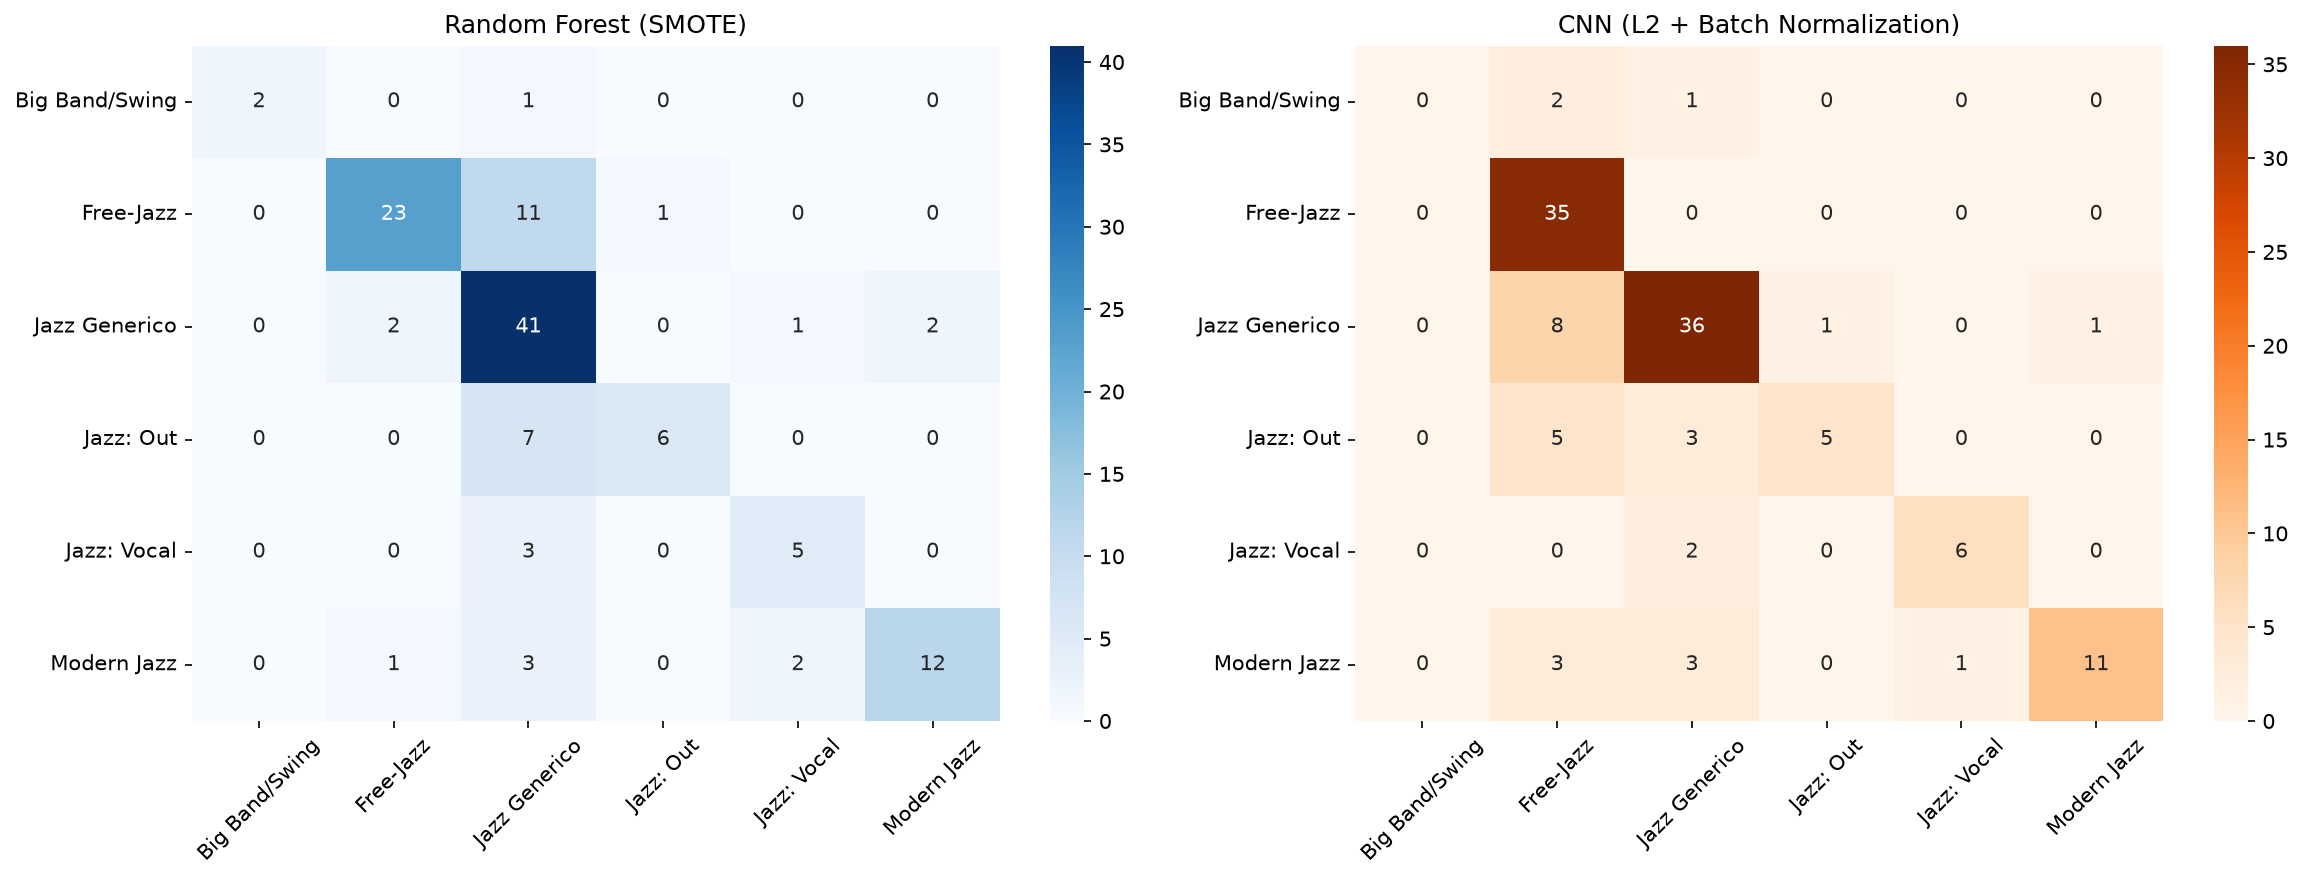
\includegraphics[width=\columnwidth]{figures/confusion_matrices.png}
% cuando se genere la figura desde el notebook
\fbox{\parbox{0.9\columnwidth}{\centering\vspace{1.5cm}
[Figura: Matrices de confusión RF (izq.) y CNN (der.)]\\
\vspace{1.5cm}}}
\caption{Matrices de confusión para el Random Forest con SMOTE (izquierda) y la CNN con regularización L2 y Batch Normalization (derecha). La CNN logra recall perfecto en Free-Jazz pero presenta dificultades en Big Band/Swing dado el escaso número de muestras de esa clase.}
\label{fig:confusion}
\end{figure}

La Fig.~\ref{fig:training} muestra las curvas de entrenamiento de la CNN. La brecha entre exactitud de entrenamiento ($\approx$75\%) y validación ($\approx$42\% en el mejor punto) evidencia overfitting a pesar de las técnicas de regularización aplicadas, lo que se atribuye principalmente al tamaño reducido del conjunto de entrenamiento.

\begin{figure}[htbp]
\centering
% Reemplazar con 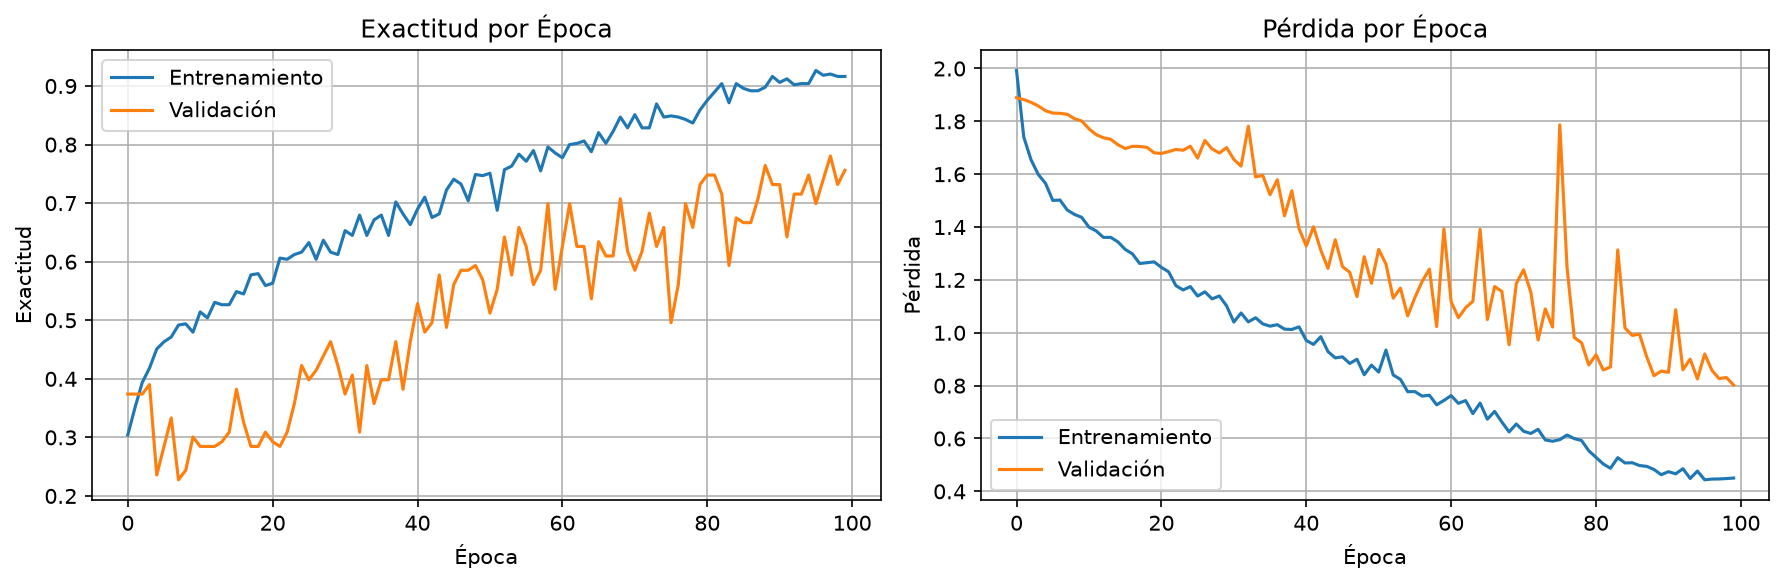
\includegraphics[width=\columnwidth]{figures/training_curves.png}
\fbox{\parbox{0.9\columnwidth}{\centering\vspace{1.5cm}
[Figura: Curvas de accuracy y loss de entrenamiento vs validación CNN]\\
\vspace{1.5cm}}}
\caption{Curvas de exactitud y pérdida por época para la CNN optimizada. El EarlyStopping restaura los pesos de la época con menor pérdida de validación.}
\label{fig:training}
\end{figure}

% ============================================================
\section{Análisis Crítico de Resultados}

\subsection{Comportamiento del Random Forest}
La aplicación de SMOTE dinámico acoplada a una búsqueda aleatoria exhaustiva (200 iteraciones) produjo un ensamble de bosques estadísticamente estable con 72\% de exactitud y F1-macro de 0.71. El modelo muestra una pauta consistente: alta precisión en casi todas las clases (86--100\%) pero recall moderado (46--89\%), lo que indica que es conservador al predecir clases minoritarias. Esto es esperado en modelos basados en árboles entrenados con SMOTE: las fronteras de decisión se trazan sobre muestras sintéticas que pueden no capturar la variabilidad real de las clases sub-representadas.

\subsection{Overfitting en la CNN y el Rol de la Regularización}
El rediseño arquitectónico de la CNN fue determinante. En iteraciones anteriores, la red sufría colapso de modo severo: primero hacia ``Modern Jazz'' y luego hacia ``Jazz Genérico'', con exactitud de prueba del 15\% y 37\% respectivamente. La combinación de reducción de capacidad, regularización L2 y eliminación de los pesos de clase resolvió el problema, elevando la exactitud al 76\%.

No obstante, la brecha entre entrenamiento y validación persiste. Con aproximadamente 490 muestras de entrenamiento distribuidas en seis clases, la CNN carece de suficientes ejemplos para generalizar bien en todas las clases. Esto se refleja en el caso de Big Band/Swing, que con solo 15 muestras originales (3 en el conjunto de prueba) obtiene F1 de 0.00 tanto en RF como en CNN. Este resultado no implica un fallo del modelo, sino una limitación inherente al tamaño del corpus para esa clase.

\subsection{La CNN como Detector de Free-Jazz}
El resultado más interesante de la CNN es su recall perfecto (1.00) en Free-Jazz, con una precisión del 66\%. Esto indica que la red aprendió a identificar los patrones espectrales caóticos y aperiódicos característicos del Free-Jazz (disonancias, estructuras polirrítmicas) con alta sensibilidad, aunque a costa de algunas predicciones falsas positivas. El RF, en cambio, logra mayor precisión (88\%) pero menor recall (66\%), lo que sugiere que los descriptores estacionarios como los MFCCs capturan el timbre del Free-Jazz pero no su variabilidad temporal completa.

\subsection{El Ensamble como Solución de Compromiso}
La combinación ponderada 35\% RF / 65\% CNN produce el mejor equilibrio entre precisión y recall en Free-Jazz (92\% precisión, 63\% recall, F1=0.75), superando a ambos modelos individuales en esta métrica. El ensamble hereda la robustez del RF en clases con pocos ejemplos y la sensibilidad espectral de la CNN en las clases dominantes, validando empíricamente la complementariedad de ambas representaciones.

% ============================================================
\section{Conclusiones y Trabajo Futuro}

La presente investigación demuestra que en las tareas de clasificación auditiva de grano fino, las decisiones de ingeniería de preprocesamiento son tan definitorias como la arquitectura de los algoritmos. La normalización de espectrogramas, la selección apropiada de la capacidad de la red y el control del overfitting mediante regularización L2 resultaron ser intervenciones más impactantes que el aumento de épocas de entrenamiento o el ajuste de hiperparámetros del optimizador.

El pipeline implementado alcanza resultados competitivos para el tamaño del corpus disponible: 76\% de exactitud con la CNN y 72\% con el ensamble, con un F1-macro de 0.71 en seis clases desequilibradas. El principal cuello de botella identificado es la escasez de ejemplos en las clases minoritarias (especialmente Big Band/Swing con 15 pistas), que limita tanto la efectividad del SMOTE como la generalización de la CNN.

Como líneas de desarrollo futuro, se plantean dos vías complementarias. La primera es la integración de arquitecturas pre-entrenadas a gran escala mediante Transfer Learning (YAMNet o AST), que permitiría aprovechar representaciones aprendidas sobre corpus de audio de millones de muestras. La segunda es la expansión del corpus mediante la incorporación de otras fuentes de datos Jazz etiquetadas, lo cual aliviaría la escasez de muestras en clases como Big Band/Swing que actualmente no pueden ser evaluadas de forma confiable.

% ============================================================
\begin{thebibliography}{00}

\bibitem{b1} M. Defferrard, K. Benzi, P. Vandergheynst, and X. Bresson, ``FMA: A Dataset for Music Analysis,'' \textit{Proceedings of the 18th International Society for Music Information Retrieval Conference (ISMIR)}, Suzhou, China, 2017.

\bibitem{b2} B. McFee et al., ``librosa: Audio and music signal analysis in python,'' in \textit{Proceedings of the 14th Python in Science Conference}, Austin, TX, 2015, pp. 18--25.

\bibitem{b3} N. V. Chawla, K. W. Bowyer, L. O. Hall, and W. P. Kegelmeyer, ``SMOTE: synthetic minority over-sampling technique,'' \textit{Journal of Artificial Intelligence Research}, vol. 16, pp. 321--357, 2002.

\bibitem{b4} S. Ioffe and C. Szegedy, ``Batch Normalization: Accelerating Deep Network Training by Reducing Internal Covariate Shift,'' \textit{Proceedings of the 32nd International Conference on Machine Learning (ICML)}, Lille, France, 2015.

\bibitem{b5} G. Tzanetakis and P. Cook, ``Musical genre classification of audio signals,'' \textit{IEEE Transactions on Speech and Audio Processing}, vol. 10, no. 5, pp. 293--302, 2002.

\bibitem{b6} K. He, X. Zhang, S. Ren, and J. Sun, ``Deep Residual Learning for Image Recognition,'' \textit{Proceedings of the IEEE Conference on Computer Vision and Pattern Recognition (CVPR)}, Las Vegas, NV, 2016.

\end{thebibliography}

\end{document}
